\begin{name}
{\tenchude}
{Trường THCS Ngọc Lâm Lần 1 Đề Chẵn \namhoc}
{\tentruong}
{\thoigian}
\end{name}

\Opensolutionfile{ansbook}[ans/THCS-NgocLam-L1-25-26-DeChan_ansbook]

\subsubsection{Câu trắc nghiệm nhiều phương án lựa chọn}
\Opensolutionfile{ans}[ans/THCS-NgocLam-L1-25-26-DeChan-TN]
% Câu trắc nghiệm nhiều phương án
\begin{ex}%[9H5H3-9]
\immini[thm]
{
Trong khoảng thời gian từ $8$ giờ đến $8$ giờ $40$ phút sáng, kim giờ của đồng hồ thực hiện một phép quay thuận chiều (với tâm ở trục quay của kim) một góc quay là bao nhiêu độ? \\
\choice
{\True $20^\circ$}
{$30^\circ$}
{$15^\circ$}
{$40^\circ$}
}
{
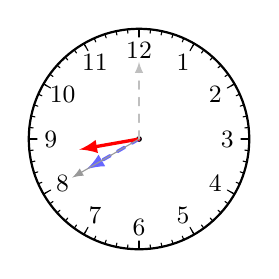
\begin{tikzpicture}[scale=.7, cap=round, >=latex]
% Vẽ mặt đồng hồ
\draw[thick, fill=white] (0,0) circle (2cm);
\fill (0,0) circle (1.5pt); % Tâm trục quay
% Vẽ vạch phút
\foreach \i in {1,...,60} {
\draw (90-\i*6:1.93cm) -- (90-\i*6:2cm);
}
% Vẽ vạch giờ và số
\foreach \i in {1,...,12} {
\draw (90-\i*30:1.85cm) -- (90-\i*30:2cm);
\node[font=\small] at (90-\i*30:1.6cm) {\i};
}
% Kim giờ lúc 8:00 (Góc -150 độ)
% 90 - 8*30 = -150
\draw[->, dashed, very thick, blue!60] (0,0) -- (-150:1.1cm) node[pos=1.35, font=\footnotesize, text=blue!80] {};
% Kim giờ lúc 8:40 (Góc -170 độ)
% 90 - (8 + 40/60)*30 = -170
\draw[->, very thick, red] (0,0) -- (-170:1.1cm) node[pos=1.35, font=\footnotesize, text=red] {};
% Cung tròn thể hiện góc quay
%	\draw[->, thick, orange] (-150:0.6cm) arc (-150:-170:0.6cm);
%	\node[orange, font=\footnotesize] at (-160:0.8cm) {$20^\circ$};
% (Tùy chọn) Kim phút làm mờ để người xem dễ hình dung ngữ cảnh thời gian
% Kim phút lúc 8:00
\draw[->, dashed, thin, gray!50] (0,0) -- (90:1.4cm);
% Kim phút lúc 8:40 (chỉ số 8)
\draw[->, thin, gray!80] (0,0) -- (-150:1.4cm);
\end{tikzpicture}
}
\loigiai{
Kim giờ quay một vòng $360^\circ$ \\
Vậy trong $1$ giờ kim quay được: $\dfrac{360^\circ}{12}=30^\circ$.\\
Từ $8$ giờ đến $8$ giờ $40$ phút là: $\dfrac{2}{3}$ giờ\\
Trong $\dfrac{2}{3}$ giờ kim quay được $30^\circ\cdot\dfrac{2}{3}=20^\circ$}
\end{ex}

\begin{ex}%[9D6N3-1]
Cho $x_1$, $x_2$ là hai nghiệm của phương trình $x^2+7x-8=0$. Khi đó $x_1+x_2$ bằng? \\
\choice
{$8$}
{$-8$}
{\True $-7$}
{$7$}
\end{ex}

\begin{ex}%[9D6H1-3]
\immini[thm]
{
Cho đồ thị hàm số $y=ax^2$ là parabol như hình vẽ bên. Khi đó giá trị của biểu thức $P=100-5a^2$ bằng
\choice
{$95$}
{$90$}
{$120$}
{\True $80$}
}
{
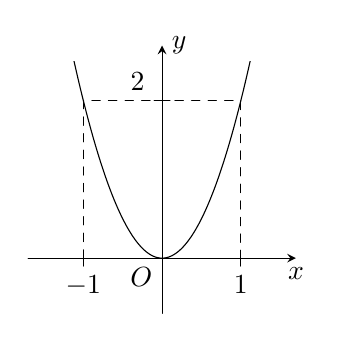
\begin{tikzpicture}[scale=1, line join=round, line cap=round, >=stealth]
\tikzset{every node/.style={scale=1}}
\def\xmin{-1.5}\def\xmax{1.5}\def\ymin{-0.5}\def\ymax{2.5}
\draw[->] (\xmin-0.2,0)--(\xmax+0.2,0) node[below]{$x$};
\draw[->] (0,\ymin-0.2)--(0,\ymax+0.2) node[right]{$y$};
\draw (0,0) node[below left]{$O$};
\foreach \x in {-1,1}\draw (\x,0.1)--(\x,-0.1) node[below]{$\x$};
\foreach \y in {2}\draw (0.1,\y)--(-0.1,\y) node[above left]{$\y$};
\clip (\xmin,\ymin) rectangle (\xmax,\ymax);
\draw[dashed] (-1,0)--(-1,2)--(0,2)--(1,2)--(1,0);
\draw[smooth,samples=200,domain=\xmin:\xmax] plot (\x,{2*((\x)^2)+0*\x+0});
\end{tikzpicture}
}
\end{ex}

\begin{ex}%[9D2H3-2]
Số giá trị nguyên dương của $x$ thỏa mãn bất phương trình $\dfrac{5x-3}{3}\le x+3$ là
\choice
{$4$}
{$7$}
{\True $6$}
{$5$}
\end{ex}

\begin{ex}%[9X8H2-2]
Gieo một con xúc xắc cân đối, đồng chất hai lần liên tiếp. Xác suất của biến cố $A$: \lq\lq Tổng số chấm xuất hiện trên con xúc xắc trong hai lần gieo bằng $10$\rq\rq\ bằng
\choice
{$\dfrac{1}{9}$}
{$\dfrac{1}{6}$}
{$\dfrac{5}{36}$}
{\True $\dfrac{1}{12}$}
\loigiai{
Không gian mẫu khi gieo hai con xúc xắc có $36$ khả năng xảy ra.\\
Biến cố $A$: \lq\lq Tổng số chấm xuất hiện trên con xúc xắc trong hai lần gieo bằng $10$\rq\rq\\
Biến cố $A$ có $3$ kết quả thuận lợi: $\left(4; 6\right);\left(5; 5\right);\left(6; 4\right)$.\\
Do đó xác suất của biến cố $A$ là: $P\left(A\right)=\dfrac{3}{36}=\dfrac{1}{12}$}
\end{ex}

\begin{ex}
\immini[thm]
{
Đài phun nước ở Công viên Hồ Khánh Hội, TP HCM vừa khánh thành vào ngày $31/08/2019$. Đài phun nước có dạng đường tròn (gọi là đường tròn tâm $(O)$) và được thiết kế theo hình dáng những cánh hoa đan xen nhau, bên dưới là hệ thống phun nước với nhiều độ cao khác nhau kết hợp với hệ thống chiếu sáng và âm nhạc cùng các mảng cây xanh tạo không gian đô thị vui tươi, sinh động. Một học sinh vẽ tam giác đều $ABC$
}
{
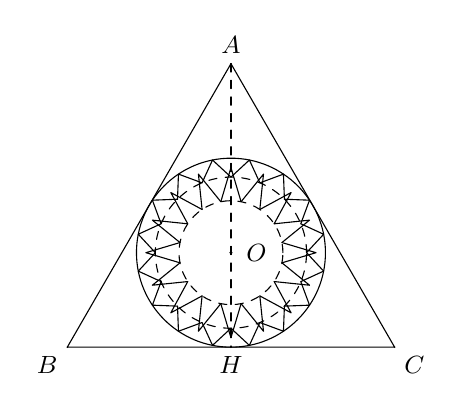
\begin{tikzpicture}[line cap=round, line join=round, >=stealth, font=\small,scale=0.6]
% Center
\coordinate (O) at (0,0);
% Define radii
\def\rout{2} % Outer circle (inscribed in triangle)
\def\rmid{1.6} % Middle dashed circle (bases of petals)
\def\rin{1.1} % Inner circle (center of flower)
\def\rpetal{1.8} % Tip of inner petals
% Triangle vertices
\coordinate (H) at (0,-\rout);
% In an equilateral triangle inscribed circle has radius r.
% The height is h = 3r, so A is at (0, 2r).
% The base is 2*r*sqrt(3), so B and C are at (-r*sqrt(3), -r) and (r*sqrt(3), -r).
% Let's use generic tangent lines to create the triangle.
% Assuming equilateral for simplicity and visual match.
\coordinate (A) at (0, 2*\rout);
\pgfmathsetmacro{\xBC}{\rout*sqrt(3)}
\coordinate (B) at (-\xBC, -\rout);
\coordinate (C) at (\xBC, -\rout);
% Draw triangle
\draw (A) -- (B) -- (C) -- cycle;
% Draw altitude/symmetry line
\draw[dashed] (A) -- (H);
% Draw circles
\draw (O) circle (\rout);
\draw[dashed] (O) circle (\rmid);
\draw[dashed] (O) circle (\rin);
% Draw petals
\def\numpetals{16}
\pgfmathsetmacro{\angleStep}{360/\numpetals}
\foreach \i in {1,...,\numpetals} {
\pgfmathsetmacro{\ang}{\i*\angleStep}
\pgfmathsetmacro{\angNext}{(\i+1)*\angleStep}
\pgfmathsetmacro{\angMid}{(\ang+\angNext)/2}
% Outer petals (tips touching outer circle)
\draw (\ang:\rmid) -- (\angMid:\rout) -- (\angNext:\rmid);
% Inner petals (tips touching rpetal circle)
\draw (\angMid:\rin) -- (\angNext:\rpetal) -- (\angNext+\angleStep/2:\rin);
}
% Labels and points
\fill (O) circle (1pt) node[right=2pt] {$O$};
\fill (A) circle (0.5pt) node[above] {$A$};
\fill (B) circle (0.5pt) node[below left] {$B$};
\fill (C) circle (0.5pt) node[below right] {$C$};
\fill (H) circle (0.5pt) node[below] {$H$};
\end{tikzpicture}
}
\noindent ngoại tiếp đường tròn $(O)$ và tính được diện tích tam giác đều là $1200\,\text{m}^2$. Bạn hãy chu vi của đường tròn $(O)$. (Kết quả làm đến hàng phần mười và $\pi = 3,14$). \\
\choice
{$94,5\,\text{cm}$}
{$96,5\,\text{cm}$}
{\True $95,5\,\text{cm}$}
{$95,59\,\text{cm}$}
\loigiai{
Kẻ $AH \perp BC$ tại $H$.\\
Tam giác đều $ABC$ ngoại tiếp đường tròn $(O)$ nên $O$ là trọng tâm của tam giác $ABC$.\\
Suy ra $O$ thuộc trung tuyến $AH$ của tam giác $ABC$.\\
Đặt $AB = a\,(\text{cm})$, ta có:\\
$AH = \dfrac{a\sqrt{3}}{2}\,(\text{cm})$; $OH = \dfrac{a\sqrt{3}}{6}\,(\text{cm})$\\
$S_{\Delta ABC} = \dfrac{a^2\sqrt{3}}{4} = 1200$\\
Suy ra $a = \sqrt{\dfrac{4.1200}{\sqrt{3}}} \approx 52,6\,(\text{cm})$.\\
Do đó $OH = \dfrac{52,6.\sqrt{3}}{6} \approx 15,2\,(\text{cm})$\\
Chu vi của đường tròn $(O)$ là $2.3,14.15,2 \approx 95,5\,(\text{cm})$.
}
\end{ex}

\begin{ex}%[9D2H3-2]
Nghiệm của bất phương trình $4x-3\le 2x+5$ là
\choice
{$x\le 1$}
{\True $x\le 4$}
{$x\ge 4$}
{$x<4$}
\end{ex}

\begin{ex}%[9H4H2-1]
\immini[thm]{
Cho tam giác $ABC$ vuông tại $A$, đường cao $AH$, biết $BH=2\text{ cm}, HC=8\text{ cm}$. Độ dài $AH$ bằng
\choice
{$16\text{ cm}$}
{$10\text{ cm}$}
{\True $4\text{ cm}$}
{$2\sqrt{5}\text{ cm}$}
}{
\begin{tikzpicture}[scale=0.8, line join=round, line cap=round, >=stealth]
\path (-1,0) coordinate (B)
(4,0) coordinate (C)
(0,0) coordinate (H)
(0,2) coordinate (A);
\draw (A)--(B)--(C)--cycle (A)--(H);
\draw pic[draw,angle radius=2mm] {right angle = B--A--C};
\draw pic[draw,angle radius=2mm] {right angle = A--H--C};
\foreach \p/\g in {A/90, B/180, C/0, H/-90}
\fill (\p) circle (1.5pt) node[shift={(\g:3mm)}]{$\p$};
\end{tikzpicture}
}
\end{ex}

\begin{ex}%[9H4N1-1]
\immini[thm]{
Cho tam giác $MNP$ vuông tại $N$. Hệ thức nào sau đây là đúng? \\
\choice
{$NP=MP\cdot\tan M$}
{$NP=MP\cdot\cos M$}
{\True $NP=MP\cdot\sin M$}
{$NP=MP\cdot\cot M$}
}{
\begin{tikzpicture}[scale=0.75, line join=round, line cap=round, >=stealth]
\path (0,0) coordinate (N)
(0,3) coordinate (M)
(4,0) coordinate (P);
\draw (N)--(M)--(P)--cycle;
\draw pic[draw,angle radius=2mm] {right angle = M--N--P};
\foreach \p/\g in {N/-135, M/90, P/0}
\fill (\p) circle (1.5pt) node[shift={(\g:3mm)}]{$\p$};
\end{tikzpicture}
}
\end{ex}

\begin{ex}%[9D3N1-2]
Điều kiện xác định của biểu thức $\sqrt{2x-6}$ là
\choice
{$x\le 3$}
{\True $x\ge 3$}
{$x\ne 3$}
{$x>3$}
\end{ex}

\begin{ex}%[9H5N3-X]
Trong một đường tròn có bán kính $R$, hình quạt tròn ứng với cung $n^\circ$ có diện tích là
\choice
{$\dfrac{\pi R^2n}{180}$}
{$\dfrac{\pi Rn}{360}$}
{$\dfrac{\pi Rn}{180}$}
{\True $\dfrac{\pi R^2n}{360}$}
\end{ex}

\begin{ex}%[9H4H2-2]
\immini[thm]{
Cho tam giác $ABC$ vuông tại $A$ có $AB=4\text{ cm}$, $\widehat{ABC}=60^\circ$. Diện tích tam giác $ABC$ bằng bao nhiêu? (làm tròn kết quả đến hàng phần trăm)
\choice
{\True $13,86\text{ cm}^2$}
{$6,93\text{ cm}^2$}
{$8\text{ cm}^2$}
{$16\text{ cm}^2$}
}{
\begin{tikzpicture}[scale=0.8, line join=round, line cap=round, >=stealth]
\path (0,0) coordinate (A)
(2,0) coordinate (B)
(0,3.464) coordinate (C);
\draw (A)--(B)--(C)--cycle;
\draw pic[draw,angle radius=2mm] {right angle = B--A--C};
\draw (1.6,0) arc (180:120:0.4);
\node at (1.2, 0.3) {$60^\circ$};
\foreach \p/\g in {A/-135, B/-45, C/90}
\fill (\p) circle (1.5pt) node[shift={(\g:3mm)}]{$\p$};
\end{tikzpicture}
}
\end{ex}

\begin{ex}%[9D1V3-0]
Bác Bình chia số tiền $800$ triệu đồng của mình cho hai khoản đầu tư. Sau một năm, tổng số tiền lãi bác thu được là $46$ triệu đồng. Lãi suất cho khoản đầu tư thứ nhất là $5\%$ /năm và khoản đầu tư thứ hai là $7\%$ /năm. Khẳng định nào sau đây đúng? \\
\choice
{Bác Bình đầu tư cho khoản thứ nhất là $600$ triệu đồng và đầu tư cho khoản thứ hai là $200$ triệu đồng}
{Bác Bình đầu tư cho khoản thứ nhất là $400$ triệu đồng và đầu tư cho khoản thứ hai là $400$ triệu đồng}
{Bác Bình đầu tư cho khoản thứ nhất là $300$ triệu đồng và đầu tư cho khoản thứ hai là $500$ triệu đồng}
{\True Bác Bình đầu tư cho khoản thứ nhất là $500$ triệu đồng và đầu tư cho khoản thứ hai là $300$ triệu đồng}
\loigiai{
Gọi số tiền đầu tư cho khoản thứ nhất và thứ hai lần lượt là $x;y$ (triệu đồng)\\
Điều kiện: $x>0;y>0$ \\
Theo bài: Tổng số tiền đầu tư là $800$ triệu đồng nên ta có phương trình: $x+y=800$ \\
Theo bài: Lãi suất cho khoản đầu tư thứ nhất là $5\%$ /năm và khoản đầu tư thứ hai là $7\%$ /năm nên ta có phương trình: $0,05x+0,07y=46$ \\
Vậy ta có hệ phương trình: $\heva{	&x+y=800\\
&0,05x+0,07y=46}$ \\
Suy ra $\heva{	&x=500\\
&y=300}$ (thoả mãn)\\
Vậy Bác Bình đầu tư cho khoản thứ nhất là $500$ triệu đồng và đầu tư cho khoản thứ hai là $300$ triệu đồng.}
\end{ex}

\begin{ex}%[9D3V3-8]
Biểu thức $M=\left(\dfrac{3}{\sqrt{x}-2}+\dfrac{3\sqrt{x}}{x-4}\right):\left(\dfrac{\sqrt{x}+1}{\sqrt{x}-2}-1\right)$ (với $x \ge 0, x \ne 4$) có kết quả rút gọn là $\dfrac{m\sqrt{x}+n}{\sqrt{x}+2}$ với $m,n$ là các số nguyên. Khi đó $m+n$ bằng
\choice
{$5$}
{\True $4$}
{$3$}
{$2$}
\loigiai{
$M=\left(\dfrac{3}{\sqrt{x}-2}+\dfrac{3\sqrt{x}}{x-4}\right):\left(\dfrac{\sqrt{x}+1}{\sqrt{x}-2}-1\right)$ \\
$M=\dfrac{3\left(\sqrt{x}+2\right)+3\sqrt{x}}{\left(\sqrt{x}-2\right)\left(\sqrt{x}+2\right)}:\dfrac{\sqrt{x}+1-\sqrt{x}+2}{\sqrt{x}-2}$ \\
$M=\dfrac{6\sqrt{x}+6}{\left(\sqrt{x}-2\right)\left(\sqrt{x}+2\right)}\cdot\dfrac{\sqrt{x}-2}{3}$ \\
$M=\dfrac{6\left(\sqrt{x}+1\right)}{3\left(\sqrt{x}+2\right)}=\dfrac{2\sqrt{x}+2}{\sqrt{x}+2}$ \\
Vì $M=\dfrac{m\sqrt{x}+n}{\sqrt{x}+2}$ nên $m=2;n=2$ \\
Có $m+n=2+2=4$}
\end{ex}

\begin{ex}%[9D1H2-4]
Hệ phương trình $\heva{	&x+2y=5\\
& x-y=2}$ có nghiệm $\left(x_0; y_0\right)$. Khi đó giá trị của biểu thức $A=1000x_0-2000y_0$ là
\choice
{$3000$}
{$-1000$}
{$2000$}
{\True $1000$}
\end{ex}

\begin{ex}%[9X7N2-3]
Giáo viên chủ nhiệm thống kê kết quả học tập cuối học kì $II$ của $40$ học sinh lớp mình. Kết quả được biểu diễn trong hình dưới đây:
\begin{center}\begin{tikzpicture}[scale=0.8]
\begin{axis}[
ybar,
title={Biểu đồ tần số tương đối kết quả học tập cuối học kì II},
xlabel={},
ylabel={\%},
ymin=0,
ymax=60,
ytick={0,10,20,30,40,50,60},
symbolic x coords={Tốt, Khá, Đạt, Chưa đạt},
xtick=data,
nodes near coords,
nodes near coords align={vertical},
bar width=0.7cm,
enlarge x limits={0.25},
ymajorgrids=true,
grid style=dashed,
ticklabel style={font=\small},
title style={font=\bfseries\small},
label style={font=\small},
legend pos=north west,
axis line style={-latex},
x tick label style={rotate=0, anchor=near xticklabel}
]
\addplot[fill=red, pattern=north east lines, pattern color=black] coordinates {
(Tốt, 20)
(Khá, 52)
(Đạt, 24)
(Chưa đạt, 4)
};
\end{axis}
\end{tikzpicture}\end{center}
Có bao nhiêu phần trăm học sinh xếp loại từ mức khá trở lên? \\
\choice
{$20\%$}
{$52\%$}
{\True $72\%$}
{$96\%$}
\loigiai{
Tỉ lệ phần trăm học sinh xếp loại từ mức khá trở lên là:\\
$20\%+52\%=72\%$}
\end{ex}

\begin{ex}%[9D3N4-1]
Căn bậc ba của $-64$ bằng
\choice
{$-4\sqrt{2}$}
{$4$}
{$-8$}
{\True $-4$}
\end{ex}

\begin{ex}%[9D2N3-1]
Bất phương trình nào sau đây không là bất phương trình bậc nhất một ẩn? \\
\choice
{\True $\dfrac{5}{x} + 1 > 0$}
{$2x + 5 \le 0$}
{$4x - 7 \ge 0$}
{$\sqrt{3}x - 2 < 0$}
\end{ex}

\begin{ex}%[9H0N2-1]
\immini[thm]{
Thể tích của hình cầu có bán kính $R$ là
\choice
{\True $\dfrac{4}{3}\pi R^3$}
{$4\pi R^2$}
{$\dfrac{1}{3}\pi R^3$}
{$\pi R^3$}
}{
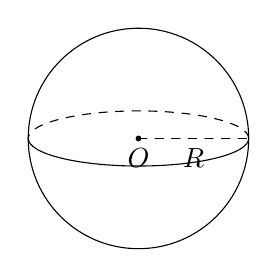
\begin{tikzpicture}[scale=0.7, line join=round, line cap=round, >=stealth]
\coordinate (O) at (0,0);
\draw (O) circle (2);
\draw[dashed] (2,0) arc (0:180:2 and 0.5);
\draw (-2,0) arc (180:360:2 and 0.5);
\fill (O) circle (1.5pt) node[below] {$O$};
\draw[dashed] (O) -- (2,0) node[midway, below] {$R$};
\end{tikzpicture}
}
\end{ex}

\begin{ex}%[9D6N1-4]
Điểm nào sau đây thuộc đồ thị hàm số $y=-\dfrac{1}{2}x^2$?
\choice
{$D\left(1;\dfrac{-1}{4}\right)$}
{\True $A\left(-2;-2\right)$}
{$C\left(4;-4\right)$}
{$B\left(-2;2\right)$}
\end{ex}

\begin{ex}%[9H0H1-2]
\immini[thm]{
Cho hình chữ nhật $ABCD$ có $AB=2\text{ cm}, BC=5\text{ cm}$. Quay hình chữ nhật $ABCD$ một vòng quanh cạnh $BC$ cố định ta được một hình trụ có diện tích xung quanh bằng
\choice
{$14\pi\text{ cm}^2$}
{$10\pi\text{ cm}^2$}
{\True $20\pi\text{ cm}^2$}
{$40\pi\text{ cm}^2$}
}{
\begin{tikzpicture}[scale=0.6, line join=round, line cap=round, >=stealth]
\def\r{2}
\def\h{4}
\coordinate (B) at (0,0);
\coordinate (C) at (0,\h);
\coordinate (A) at (\r,0);
\coordinate (D) at (\r,\h);
\draw[dashed] (0,-1) -- (0,\h+1);
\draw[thick,dashed, pattern=north east lines] (A)--(B)--(C)--(D)--cycle;
\draw (A)--(D);
\draw (-\r,0) -- (-\r,\h);
\draw[dashed] (\r,0) arc (0:180:\r cm and 0.5cm);
\draw (-\r,0) arc (180:360:\r cm and 0.5cm);
\draw[] (\r,\h) arc (0:180:\r cm and 0.5cm);
\draw (-\r,\h) arc (180:360:\r cm and 0.5cm);
\foreach \p/\g in {A/0, B/225, C/135, D/0}
\fill (\p) circle (1.5pt) node[shift={(\g:3mm)}]{$\p$};
\end{tikzpicture}
}
\end{ex}

\begin{ex}%[9D2N3-3]
Gọi $x\left(x\in\mathbb{N}\right)$ là số học sinh trong lớp. Bất đẳng thức nào sau đây mô tả tình huống \lq\lq Trong lớp có ít nhất $20$ học sinh\rq\rq? \\
\choice
{\True $x\ge 20$}
{$x<20$}
{$x>20$}
{$x\le 20$}
\end{ex}

\begin{ex}%[9X7N2-2]
Giáo viên chủ nhiệm lớp $9A$ thực hiện khảo sát về phương tiện đi học của học sinh trong lớp. Kết quả khảo sát được trình bày như sau:
\begin{table}[h!]
\centering
\caption{Thống kê phương tiện di chuyển}
\renewcommand{\arraystretch}{1.2}
\begin{tabular}{|l|c|c|c|c|}
\hline
\textbf{Phương tiện} & \textbf{Xe đạp} & \textbf{Xe đạp điện} & \textbf{Xe buýt} & \textbf{Phương tiện khác} \\
\hline
Tần số ($n$) & $20$ & $10$ & $8$ & $5$ \\
\hline
Tần số tương đối $f$ (\%) & $50$ & $25$ & $20$ & $5$ \\
\hline
\end{tabular}
\end{table}
Tỉ lệ phần trăm học sinh đi xe đạp điện là
\choice
{$20\%$}
{\True $25\%$}
{$50\%$}
{$10\%$}
\end{ex}

\begin{ex}%[9X8H1-1]
Bạn Bình gieo một con xúc xắc cân đối và đồng chất hai lần liên tiếp. Số phần tử của không gian mẫu là
\choice
{$6$}
{\True $36$}
{$12$}
{$24$}
\end{ex}

\begin{ex}%[9H4N1-1]
Cho tam giác $ABC$ vuông tại $A$ có $AC=3\text{ cm}, BC=5\text{ cm}$. Khẳng định nào sau đây đúng? \\
\choice
{\True $\sin B=\dfrac{3}{5}$}
{$\sin B=\dfrac{4}{5}$}
{$\tan B=\dfrac{4}{5}$}
{$\cos B=\dfrac{3}{5}$}
\loigiai{
Tam giác $ABC$ vuông tại $A$ có $\sin B=\dfrac{AC}{BC}=\dfrac{3}{5}$}
\end{ex}

\begin{ex}%[9D6V3-6]
Cho parabol $\left(P\right)\colon y=x^2$ và đường thẳng $(d)\colon y=4x-m+1$. Số giá trị của $m$ để $\left(P\right)$ và $(d)\colon$ cắt nhau tại hai điểm phân biệt có hoành độ $x_1$, $x_2$ thỏa mãn điều kiện $x_1^2x_2+x_1x_2^2=-8$ là
\choice
{\True $1$}
{$0$}
{$3$}
{$2$}
\end{ex}
\Closesolutionfile{ans}

\subsubsection{Câu trắc nghiệm đúng sai}
\Opensolutionfile{ans}[ans/THCS-NgocLam-L1-25-26-DeChan-DS]
% Câu trắc nghiệm đúng sai
\begin{ex}%[9D6V3-5]
Cho phương trình bậc hai $x^2-2(m-1)x+m+1=0$ (1) (ẩn $x$, tham số $m$ ). \\
\choiceTF
{Hệ số của $x$ trong phương trình (1) là $2(m-1)$}
{\True Phương trình (1) luôn có hai nghiệm trái dấu khi $m<-1$}
{\True Khi $m=3$ thì phương trình (1) có nghiệm kép}
{Không có giá trị của $m$ để hai nghiệm $x_1, x_2$ của phương trình (1) là độ dài hai cạnh góc vuông của một tam giác vuông có diện tích bằng $4$ (đvdt)}
\loigiai{
\begin{itemchoice}
\itemch Hệ số của $x$ trong phương trình (1) là $-2(m-1)$. \\ Vậy mệnh đề sai. \\
\itemch Phương trình (1) có hai nghiệm trái dấu khi $1 \cdot (m+1) < 0$. Hay $m < -1$. \\ Vậy mệnh đề đúng. \\
\itemch Phương trình (1) có nghiệm kép khi \\
$\Delta' = 0 \Rightarrow [-(m-1)]^2 - 1 \cdot (m+1) = 0 \Rightarrow m^2 - 2m + 1 - m - 1 = 0 \Rightarrow m^2 - 3m = 0 \Rightarrow \left[\begin{array}{l}m=0 \\ m=3\end{array}\right.$.\\
Vậy $m=3$ thì phương trình (1) có nghiệm kép. \\ Vậy mệnh đề đúng. \\
Phương trình (1) có hai nghiệm $x_1, x_2$ khi \\
$\Delta' > 0 \Rightarrow (m-1)^2 - (m+1) > 0 \Rightarrow m^2-3m > 0 \Rightarrow \left[\begin{array}{l}m<0 \\ m>3\end{array}\right.$.\\
Để hai nghiệm $x_1, x_2$ của phương trình (1) là độ dài hai cạnh góc vuông của một tam giác vuông có diện tích bằng $4\,(\text{đvdt})$ thì \\
$\left\{\begin{array}{l}x_1>0, x_2>0 \\ \dfrac{1}{2}x_1 x_2 = 4\end{array}\right. \Rightarrow \left\{\begin{array}{l}x_1+x_2>0 \\ x_1 x_2 = 8\end{array}\right. \Rightarrow \left\{\begin{array}{l}2(m-1)>0 \\ m+1=8\end{array}\right. \Rightarrow \left\{\begin{array}{l}m>1 \\ m=7\end{array}\right. \Rightarrow m=7\,(\text{tmdk})$. \\ Vậy mệnh đề sai. \\
\end{itemchoice}
}
\end{ex}

\begin{ex}
Cho hai biểu thức $A = \dfrac{\sqrt{x}+3}{\sqrt{x}+1}$ và $B = \dfrac{\sqrt{x}}{\sqrt{x}-2} + \dfrac{\sqrt{x}+2}{3-\sqrt{x}} - \dfrac{x-3\sqrt{x}+5}{x-5\sqrt{x}+6}$ với $x \ge 0; x \ne 4; x \ne 9$.
\choiceTF
{\True Khi $x=25$, giá trị của biểu thức $A$ là $\dfrac{4}{3}$}
{Biểu thức $B$ sau khi rút gọn là $\dfrac{\sqrt{x}+3}{\sqrt{x}+2}$}
{\True Biểu thức $P = A:B$ có dạng rút gọn là $\dfrac{\sqrt{x}-2}{\sqrt{x}+1}$}
{Phương trình $2P = 2\sqrt{x}-9$ có nghiệm duy nhất là $x=16$}
\loigiai{
\begin{itemchoice}
\itemch Với $x=25$ (thỏa mãn điều kiện $x \ge 0$), ta thay vào biểu thức $A$: \\
$A = \dfrac{\sqrt{25}+3}{\sqrt{25}+1} = \dfrac{5+3}{5+1} = \dfrac{8}{6} = \dfrac{4}{3}$. \\
Vậy mệnh đề là đúng. \\
\itemch Điều kiện xác định: $x \ge 0; x \ne 4; x \ne 9$. \\
Ta có $3-\sqrt{x} = -(\sqrt{x}-3)$ và $x-5\sqrt{x}+6 = (\sqrt{x}-2)(\sqrt{x}-3)$. \\
$B = \dfrac{\sqrt{x}}{\sqrt{x}-2} + \dfrac{\sqrt{x}+2}{3-\sqrt{x}} - \dfrac{x-3\sqrt{x}+5}{x-5\sqrt{x}+6}$ \\
$B = \dfrac{\sqrt{x}}{\sqrt{x}-2} - \dfrac{\sqrt{x}+2}{\sqrt{x}-3} - \dfrac{x-3\sqrt{x}+5}{(\sqrt{x}-2)(\sqrt{x}-3)}$ \\
Quy đồng mẫu số chung là $(\sqrt{x}-2)(\sqrt{x}-3)$: \\
$B = \dfrac{\sqrt{x}(\sqrt{x}-3) - (\sqrt{x}+2)(\sqrt{x}-2) - (x-3\sqrt{x}+5)}{(\sqrt{x}-2)(\sqrt{x}-3)}$ \\
$B = \dfrac{(x-3\sqrt{x}) - (x-4) - (x-3\sqrt{x}+5)}{(\sqrt{x}-2)(\sqrt{x}-3)}$ \\
$B = \dfrac{x-3\sqrt{x} - x+4 - x+3\sqrt{x}-5}{(\sqrt{x}-2)(\sqrt{x}-3)}$ \\
$B = \dfrac{-x-1}{(\sqrt{x}-2)(\sqrt{x}-3)}$. \\
Vậy mệnh đề là sai. \\
\itemch Ta có $P = A:B$. Sử dụng kết quả rút gọn $B = \dfrac{\sqrt{x}+3}{\sqrt{x}-2}$ từ bài giải đã cho: \\
$P = \dfrac{\sqrt{x}+3}{\sqrt{x}+1} : \dfrac{\sqrt{x}+3}{\sqrt{x}-2}$ \\
$P = \dfrac{\sqrt{x}+3}{\sqrt{x}+1} \cdot \dfrac{\sqrt{x}-2}{\sqrt{x}+3}$ \\
$P = \dfrac{\sqrt{x}-2}{\sqrt{x}+1}$ (với điều kiện $x \ne 9$ để $\sqrt{x}+3 \ne 0$). \\
Vậy mệnh đề là đúng. \\
Thay $P = \dfrac{\sqrt{x}-2}{\sqrt{x}+1}$ vào phương trình $2P = 2\sqrt{x}-9$: \\
$2 \cdot \dfrac{\sqrt{x}-2}{\sqrt{x}+1} = 2\sqrt{x}-9$ \\
$2(\sqrt{x}-2) = (2\sqrt{x}-9)(\sqrt{x}+1)$ \\
$2\sqrt{x}-4 = 2x + 2\sqrt{x} - 9\sqrt{x} - 9$ \\
$2\sqrt{x}-4 = 2x - 7\sqrt{x} - 9$ \\
$2x - 9\sqrt{x} - 5 = 0$ \\
Đặt $t = \sqrt{x}$ ($t \ge 0$). Phương trình trở thành $2t^2 - 9t - 5 = 0$. \\
Giải phương trình bậc hai: $\Delta = (-9)^2 - 4(2)(-5) = 81 + 40 = 121 = 11^2$. \\
$t_1 = \dfrac{9-11}{4} = -\dfrac{2}{4} = -\dfrac{1}{2}$ (loại vì $t \ge 0$). \\
$t_2 = \dfrac{9+11}{4} = \dfrac{20}{4} = 5$ (nhận). \\
Với $t=5$, ta có $\sqrt{x}=5 \Rightarrow x=25$. \\
Giá trị $x=25$ thỏa mãn điều kiện xác định ($x \ge 0; x \ne 4; x \ne 9$). \\
Vậy phương trình có nghiệm duy nhất là $x=25$, không phải $x=16$. \\
Mệnh đề là sai. \\
\end{itemchoice}
}
\end{ex}
\Closesolutionfile{ans}

\subsubsection{Câu trắc nghiệm trả lời ngắn}
\Opensolutionfile{ans}[ans/THCS-NgocLam-L1-25-26-DeChan-TLN]
% Câu trắc nghiệm trả lời ngắn
\begin{ex}%[9D3V3-4]
Biểu thức $\dfrac{\sqrt{3}+\sqrt{2}}{\sqrt{3}-\sqrt{2}}$ được rút gọn dưới dạng $a+b\sqrt{6}$ (với $a,b$ là các số nguyên). Tính giá trị của $P=a-b$.\\
\shortans{$3$}
\loigiai{
Ta có $\dfrac{\sqrt{3}+\sqrt{2}}{\sqrt{3}-\sqrt{2}} = \dfrac{(\sqrt{3}+\sqrt{2})^2}{(\sqrt{3}-\sqrt{2})(\sqrt{3}+\sqrt{2})} = \dfrac{3+2\sqrt{6}+2}{3-2} = 5+2\sqrt{6}$.\\
Đối chiếu với $a+b\sqrt{6}$, ta có $a=5$ và $b=2$.\\
Vậy $P = a-b = 5-2 = 3$.
}
\end{ex}

\begin{ex}%[9H5H2-3]
Cho đường tròn $(O)$ có đường kính bằng $16\text{cm}$. Bán kính của đường tròn này bằng bao nhiêu cm?\\
\shortans{$8$}
\loigiai{
Bán kính đường tròn bằng một nửa đường kính: $R = 16:2 = 8\text{cm}$.
}
\end{ex}

\begin{ex}%[9H4V2-5]
Một người đứng cách chân một cột cờ $15\text{m}$, nhìn thấy đỉnh cột cờ dưới một góc $42^\circ$ so với phương nằm ngang. Biết mắt người đó cách mặt đất $1,6\text{m}$. Chiều cao của cột cờ bằng bao nhiêu mét? (Làm tròn kết quả đến hàng đơn vị).\\
\shortans{$15$}
\loigiai{
Gọi $h$ là chiều cao cột cờ, $BE$ là khoảng cách từ người đến cột cờ, $BE=15\text{m}$.\\
Gọi $A$ là chân cột cờ, $C$ là đỉnh cột cờ. Điểm $B$ trên cột cờ ngang với tầm mắt người quan sát $E$.\\
Khi đó $AB$ chính là chiều cao từ mặt đất đến mắt người, $AB=1,6\text{m}$.\\
Góc nhìn đỉnh cột cờ là $\widehat{CEB}=42^\circ$.\\
Trong tam giác $CBE$ vuông tại $B$, ta có $BC = BE \cdot \tan 42^\circ = 15 \cdot \tan 42^\circ \approx 13,506\text{m}$.\\
Chiều cao cột cờ là $AC = AB + BC = 1,6 + 13,506 = 15,106\text{m}$.\\
Làm tròn đến hàng đơn vị ta được $15\text{m}$.
}
\end{ex}

\begin{ex}
\immini[thm]
{
Cho nửa đường tròn tâm $D$, đường kính $AB$. Vẽ nửa đường tròn đường kính $AD$ nằm cùng phía với nửa đường tròn đã cho. Kẻ dây cung $AC$ của nửa đường tròn lớn tạo với $AB$ một góc $30^\circ$ ($C$ thuộc nửa đường tròn lớn). Gọi $(H)$ là phần hình phẳng được giới hạn bởi đoạn thẳng $DB$, cung tròn $BC$,
}
{
\begin{tikzpicture}[scale=0.6,line join=round, line cap=round, >=Stealth]
% Định nghĩa bán kính
\def\R{4}
% Tọa độ các điểm chính trên trục hoành
\coordinate (A) at (0,0);
\coordinate (D) at (\R,0);
\coordinate (B) at (2*\R,0);
% Tâm của cung nhỏ (AD) và cung lớn (AB)
\coordinate (O1) at (\R/2,0); % Tâm cung nhỏ
\coordinate (O2) at (\R,0); % Tâm cung lớn (chính là điểm D)
% Tính toán tọa độ điểm C và E
% Đường thẳng từ A tạo góc 30 độ so với AB
% Điểm C nằm trên cung lớn (bán kính R, tâm O2)
% Điểm E là giao của AC và cung nhỏ (bán kính R/2, tâm O1)
\coordinate (C) at ({\R + \R*cos(60)}, {\R*sin(60)});
\coordinate (E) at ({\R/2 + \R/2*cos(60)}, {\R/2*sin(60)});
% 1. Vẽ phần gạch chéo (H)
\fill[pattern=north east lines, pattern color=black!70]
(D) -- (B)
arc (0:60:\R)
-- (E)
arc (60:0:\R/2)
-- cycle;
% 2. Vẽ các cung tròn và đoạn thẳng bao quanh
\draw (A) -- (B);
\draw (A) -- (C);
\draw (B) arc (0:180:\R); % Semicircle lớn AB
\draw (D) arc (0:180:\R/2); % Semicircle nhỏ AD
% 3. Ký hiệu góc 30 độ
\draw (0.8,0) arc (0:30:0.8);
\node at (1.2,0.25) {\footnotesize $30^\circ$};
% 4. Đánh dấu điểm và nhãn
\foreach \p/\pos in {A/below left, D/below, B/below right, C/above right}
\fill (\p) circle (1.5pt) node[\pos] {$\p$};
% Nhãn vùng (H)
\node at (5.5, 1.2) {\large \textbf{(H)}};
\end{tikzpicture}
}
\noindent đoạn thẳng $EC$ (với $E$ là giao điểm của $AC$ và nửa đường tròn nhỏ) và cung tròn $ED$ của nửa đường tròn nhỏ (phần gạch sọc trong hình vẽ). Tính tỉ số giữa diện tích phần gạch sọc $(H)$ và diện tích phần không gạch sọc của nửa đường tròn đường kính $AB$(làm tròn đến chữ số thập phân thứ 2). \\
\shortans{$0,84$}
\loigiai{
Giả sử bán kính nửa đường tròn lớn là $R$. Khi đó $AD = DB = R$. Diện tích nửa đường tròn lớn là $S = \dfrac{1}{2} \pi R^2$.\\
Nửa đường tròn nhỏ có đường kính $AD = R$ nên có bán kính $r = \dfrac{R}{2}$, gọi tâm là $O_1$.\\
Gọi $E$ là giao điểm của $AC$ với nửa đường tròn nhỏ. Trong nửa đường tròn nhỏ, xét tam giác $AO_1E$ có $AO_1 = O_1E = \dfrac{R}{2}$ và $\widehat{O_1AE} = 30^\circ$, suy ra $\widehat{AO_1E} = 180^\circ - 2 \cdot 30^\circ = 120^\circ$.\\
Từ đó $\widehat{DO_1E} = 180^\circ - 120^\circ = 60^\circ$.\\
Phần diện tích nửa đường tròn nhỏ nằm dưới dây cung $AC$ là tổng diện tích hình quạt $DO_1E$ và tam giác $AO_1E$.\\
Diện tích hình quạt $DO_1E$ là $S_1 = \dfrac{60}{360} \pi \left(\dfrac{R}{2}\right)^2 = \dfrac{\pi R^2}{24}$.\\
Diện tích tam giác $AO_1E$ là $S_2 = \dfrac{1}{2} \cdot \dfrac{R}{2} \cdot \dfrac{R}{2} \cdot \sin\left(120^\circ\right) = \dfrac{\sqrt{3} R^2}{16}$.\\
Tổng diện tích phần nửa đường tròn nhỏ nằm dưới $AC$ là $S_3 = S_1 + S_2 = \dfrac{\pi R^2}{24} + \dfrac{\sqrt{3} R^2}{16}$.\\
Xét nửa đường tròn lớn, tam giác $ADC$ có $DA = DC = R$ và $\widehat{DAC} = 30^\circ$, suy ra $\widehat{ADC} = 120^\circ$.\\
Góc $\widehat{CDB} = 180^\circ - 120^\circ = 60^\circ$.\\
Diện tích phần hình phẳng nằm dưới dây $AC$ của nửa đường tròn lớn bao gồm diện tích tam giác $ADC$ và hình quạt $DBC$.\\
Diện tích tam giác $ADC$ là $S_4 = \dfrac{1}{2} R^2 \sin\left(120^\circ\right) = \dfrac{\sqrt{3} R^2}{4}$.\\
Diện tích hình quạt $DBC$ là $S_5 = \dfrac{60}{360} \pi R^2 = \dfrac{\pi R^2}{6}$.\\
Diện tích phần gạch sọc $(H)$ chính là diện tích phần nằm dưới dây $AC$ của nửa đường tròn lớn trừ đi phần diện tích nửa đường tròn nhỏ nằm dưới $AC$:\\
$S_{(H)} = \left(S_4 + S_5\right) - S_3 = \left( \dfrac{\sqrt{3} R^2}{4} + \dfrac{\pi R^2}{6} \right) - \left( \dfrac{\pi R^2}{24} + \dfrac{\sqrt{3} R^2}{16} \right) = \dfrac{\pi R^2}{8} + \dfrac{3\sqrt{3} R^2}{16}$.\\
Diện tích phần không gạch sọc là $S_{kg} = S - S_{(H)} = \dfrac{1}{2} \pi R^2 - \left( \dfrac{\pi R^2}{8} + \dfrac{3\sqrt{3} R^2}{16} \right) = \dfrac{3\pi R^2}{8} - \dfrac{3\sqrt{3} R^2}{16}$.\\
Tỉ số diện tích phần gạch sọc và phần không gạch sọc là:\\
$\dfrac{S_{(H)}}{S_{kg}} = \dfrac{\dfrac{\pi}{8} + \dfrac{3\sqrt{3}}{16}}{\dfrac{3\pi}{8} - \dfrac{3\sqrt{3}}{16}} = \dfrac{2\pi + 3\sqrt{3}}{6\pi - 3\sqrt{3}}$.
}
\end{ex}

\begin{ex}%[9H5C3-8]
Cho một hình vuông $ABCD$ có cạnh bằng $10\text{cm}$. Vẽ một đường tròn tâm $O$ (là giao điểm hai đường chéo) có bán kính $R=3\text{cm}$. Tính diện tích phần hình vuông nằm ngoài đường tròn đó. (Lấy $\pi \approx 3,14$, làm tròn đến hàng phần mười).\\
\shortans{$71,7$}
\loigiai{
Diện tích hình vuông $ABCD$ là $S_{hv} = 10 \cdot 10 = 100\text{cm}^2$.\\
Diện tích hình tròn tâm $O$ bán kính $3\text{cm}$ là $S_{tr} = \pi R^2 \approx 3,14 \cdot 3^2 = 28,26\text{cm}^2$.\\
Diện tích phần nằm ngoài đường tròn là $S = S_{hv} - S_{tr} = 100 - 28,26 = 71,74\text{cm}^2$.\\
Làm tròn đến hàng phần mười ta được $71,7\text{cm}^2$.
}
\end{ex}

\begin{ex}%[9D6V4-2]
Một xưởng may theo kế hoạch cần may $600$ bộ quần áo trong một thời gian quy định. Khi thực hiện được $400$ bộ, xưởng đã cải tiến kỹ thuật nên mỗi ngày may thêm được $10$ bộ so với dự định, vì thế xưởng đã hoàn thành công việc sớm hơn $1$ ngày so với kế hoạch. Hỏi theo dự định ban đầu, mỗi ngày xưởng may được bao nhiêu bộ quần áo?\\
\shortans{$40$}
\loigiai{
Gọi năng suất dự định của xưởng mỗi ngày là $x~\text{bộ quần áo}$; $(x>0)$.\\
Thời gian dự định hoàn thành là $\dfrac{600}{x}~\text{ngày}$.\\
Thời gian may $400$ bộ đầu tiên là $\dfrac{400}{x}~\text{ngày}$.\\
Năng suất thực tế sau khi cải tiến là $x+10~\text{bộ/ngày}$.\\
Thời gian may $600-400=200$ bộ còn lại là $\dfrac{200}{x+10}~\text{ngày}$.\\
Vì xưởng hoàn thành sớm $1$ ngày nên ta có phương trình:\\
$\dfrac{400}{x} + \dfrac{200}{x+10} + 1 = \dfrac{600}{x}$\\
$\Rightarrow \dfrac{200}{x} - \dfrac{200}{x+10} = 1$\\
$\Rightarrow 200(x+10) - 200x = x(x+10)$\\
$\Rightarrow x^2 + 10x - 2000 = 0$\\
Giải phương trình ta được $x_1=40$ (thỏa mãn) và $x_2=-50$ (loại).\\
Vậy mỗi ngày xưởng dự định may $40$ bộ quần áo. \\
}
\end{ex}
\Closesolutionfile{ans}

\Closesolutionfile{ansbook}

% BẢNG ĐÁP ÁN
\indapan{THCS-NgocLam-L1-25-26-DeChan-TN}{THCS-NgocLam-L1-25-26-DeChan-DS}{THCS-NgocLam-L1-25-26-DeChan-TLN}